\begin{figure}[!ht]
    \centering
        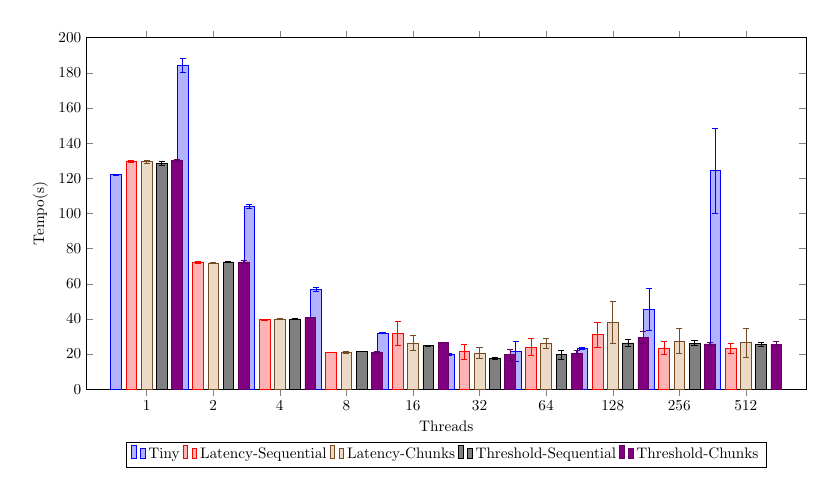
\begin{tikzpicture}[scale=0.55, baseline]
        \begin{axis}[
            width=1.5 \linewidth,
            height=0.8 \linewidth,
            %media de tempo intruder
            ybar=3pt,
            %enlargelimits=0.10,
            legend style={at={(0.5,-0.15)}, anchor=north, legend columns=-1},
            ylabel=Tempo(s),
            xlabel=Threads,
            symbolic x coords={1, 2, 4, 8, 16, 32, 64, 128, 256, 512},
            xtick=data,
            ymin=0,
            ymax=200,
            bar width=7pt,
            % nodes near coords,
            nodes near coords align={vertical},
        ]
        \addplot+[error bars,y dir=both, y explicit] coordinates {
            (1,122.19)+-(1,0.35) (2,184.47)+-(2,3.93) (4,103.92)+-(4,1.04) (8,56.80)+-(8,1.07) (16,31.99)+-(16,0.24) (32,19.69)+-(32,0.52) (64,21.68)+-(64,5.72) (128,23.22)+-(128,0.57) (256,45.58)+-(256,11.99) (512,124.45)+-(512,24.20) 
        };
        \addplot+[error bars,y dir=both, y explicit] coordinates {
            (1,129.87)+-(1,0.52) (2,72.20)+-(2,0.44) (4,39.59)+-(4,0.19) (8,21.14)+-(8,0.09) (16,31.78)+-(16,6.87) (32,21.39)+-(32,4.41) (64,24.02)+-(64,4.93) (128,31.01)+-(128,7.24) (256,23.53)+-(256,3.50) (512,23.21)+-(512,3.03)
        };
        \addplot+[error bars,y dir=both, y explicit] coordinates {
            (1,129.58)+-(1,0.88) (2,71.87)+-(2,0.48) (4,39.90)+-(4,0.39) (8,21.15)+-(8,0.64) (16,26.35)+-(16,4.18) (32,20.69)+-(32,3.15) (64,26.17)+-(64,3.04) (128,38.12)+-(128,12.03) (256,27.50)+-(256,7.32) (512,26.48)+-(512,8.21)
        };
        \addplot+[error bars,y dir=both, y explicit] coordinates {
            (1,128.56)+-(1,0.95) (2,72.45)+-(2,0.41) (4,40.00)+-(4,0.22) (8,21.55)+-(8,0.22) (16,24.76)+-(16,0.20) (32,17.51)+-(32,0.39) (64,19.62)+-(64,2.71) (128,26.34)+-(128,1.81) (256,26.30)+-(256,1.52) (512,25.59)+-(512,1.05) 
        };
        \addplot+[error bars,y dir=both, y explicit] coordinates {
            (1,130.29)+-(1,0.63) (2,72.49)+-(2,0.59) (4,40.83)+-(4,0.31) (8,21.11)+-(8,0.63) (16,26.56)+-(16,0.15) (32,19.76)+-(32,3.23) (64,20.45)+-(64,1.74) (128,29.49)+-(128,3.46) (256,25.76)+-(256,0.95) (512,25.70)+-(512,1.49)
        };
    \legend {Tiny, Latency-Sequential, Latency-Chunks, Threshold-Sequential, Threshold-Chunks}
        \end{axis}
        \end{tikzpicture}
    \caption{Tempo de execução em segundos do benchmark Vacation variando o número de \emph{threads}.}
    \label{vacation_tempo}

\end{figure}
